% !TeX root = Documentation-HU-formatted.tex

\documentclass[12pt,a4paper,hungarian]{report} 

\usepackage[utf8]{inputenc}
\usepackage[provide=*]{babel}
\usepackage{microtype}
\usepackage{graphicx}
\usepackage[utf8]{inputenc}

\title{Smart Turntable Assistant}
\author{Daniel Kiss}
\date{\today}

\clubpenalty=100000
\widowpenalty=100000

\begin{document} 
\sloppy

\maketitle
\tableofcontents

\chapter{Bevezetés}

\section{Témaválasztás indoklása}
Az elmúlt években a zeneiparban megfigyelhető a fizikai, analóg hordozók, különösen a bakelitlemezek népszerűségének jelentős visszatérése. Az audiofileket és a hétköznapi hallgatókat egyaránt vonzza a mechanikus élmény és az analóg hangzás egyedi jellemzői. Ugyanakkan a modern digitális zenehallgatási környezet (mint a Spotify vagy az Apple Music) és a hagyományos lemezjátszó használata két teljesen különálló világ maradt. 

A témát azért választottam, mert létezik egy jelentős technológiai szakadék az analóg audio jel és a modern metaadat-kezelés között. Egy olyan eszköz létrehozása, amely képes hidat képezni a fizikai lemezjátszó és a digitális kényelmi funkciók között, nemcsak technikai kihívást jelent a valós idejű jelfeldolgozás terén, hanem valódi hozzáadott értéket nyújt a hobbizáló zenehallgatók számára, akik nem szeretnének lemondni az analóg élményről, de igényelnék a digitális kor előnyeit.

\section{A megoldandó feladat leírása}
A projekt célja egy olyan „Okos Lemezjátszó Asszisztens” szoftveres rendszer megvalósítása, amely passzívan figyeli egy szabványos lemezjátszó audio kimenetét, és automatikusan nyújt digitális kiegészítéseket a hallgatáshoz.

A rendszernek a következő alapvető feladatokat kell megoldania:
\begin{itemize}
    \item \textbf{Automatikus felismerés:} A bejövő analóg jel alapján meg kell határozni, hogy egy zeneszám kezdődött-e, majd audio fingerprinting segítségével azonosítania kell a pontos előadót és dalcímet.
    \item \textbf{Metaadat-szinkronizáció:} A felismerést követően a rendszernek lekérdeznie kell a számhoz tartozó albumborítót és a szinkronizált dalszöveget, majd azt valós időben megjelenítenie kell a felhasználónak.
    \item \textbf{Hardveres monitorozás:} A szoftvernek matematikai elemzéssel nyomon kell követnie a hangszedő (tű) kopását a lejátszási órák alapján, valamint diagnosztikai adatokat (pl. motorrezgés, felületi zaj) kell szolgáltatnia.
    \item \textbf{Digitális naplózás:} A hallgatási élményt automatikusan szinkronizálnia kell külső platformokkal (pl. Last.fm), így az analóg lejátszás is digitális nyomon követhetővé válik.
\end{itemize}

\chapter{Felhasználói dokumentáció}

\section{A megoldott probléma megfogalmazása}
A hagyományos bakelitlemez-lejátszó legnagyobb hátránya, hogy a generált jel egy nyers elektromos jel, amely nem tartalmaz metaadatokat. Ez azt jelenti, hogy a felhasználó számára nincs automatikus módja a lejátszott számok naplózására, nincs hozzáférése a szinkronizált dalszövegekhez, és nincs pontos eszköze a tű kopásának vagy a lemezjátszó technikai állapotának ellenőrzésére. A Smart Turntable Assistant ezen „információs vakpontot” törli el egy intelligens szoftverréteg bevezetésével.

\section{A felhasznált módszerek rövid leírása}
A rendszer egy kliens-szerver architektúrán alapul, ahol a backend és a frontend különálló egységekben működnek:
\begin{itemize}
    \item \textbf{Audio elemzés és azonosítás:} A Python nyelvű backend a \texttt{sounddevice} és \texttt{NumPy} könyvtárakat használja a jel feldolgozásához. A számok azonosításához külső Audio Fingerprinting API-kat (pl. ACRCloud/Shazam) alkalmaz a rendszer, amelyek egyedi akusztikai „ujjlenyomatokat” hasonlítanak össze egy globális adatbázissal.
    \item \textbf{Valós idejű kommunikáció:} A szerver és a felhasználói felület közötti adatcsere WebSockets (Socket.IO) technológiával történik, ami lehetővé teszi, hogy a diagnosztikai adatok és a dalszövegek késleltetés nélkül érkezzenek a képernyőre.
    \item \textbf{Felhasználói felület:} Egy modern, reaktív weboldal (Vue.js SPA), amely bármilyen eszközön (mobil, asztali) elérhető és dinamikusan változtatja a megjelenítést a lejátszott album borítójához.
    \item \textbf{Adatkezelés:} Az SQLite adatbázis tárolja a felhasználói beállításokat és a tű élettartomát, így a rendszerbe jelentkezve a felhasználó mindig a saját konfigurációját kapja vissza.
\end{itemize}

\section{A program használatához szükséges információk}

\subsection{Telepítés és Indítás}
A program Docker konténerben fut, ami egyszerűsíti a telepítést. A futtatáshoz szükség van egy USB audio interfészre, amelyhez csatlakoztatva van a lemezjátszó.
\begin{enumerate}
    \item A Docker image letöltése és a konténer indítása a mellékelt \texttt{docker-compose.yml} fájllal.
    \item A böngészőben a \texttt{http://localhost:5000} (vagy a szerver IP címe) megnyitása.
\end{enumerate}

\subsection{Alapvető Funkciók Használata}
\begin{itemize}
    \item \textbf{Zenehallgatás:} Helyezze a tűt a lemezre. A rendszer automatikusan érzékeli a hangot, azonosítja a számot és megjeleníti az albumborítót valamint a dalszöveget.
    \item \textbf{Hangszedő regisztrálása:} A profil menüben adja meg az új tű típusát és az ajánlott élettartamát. A rendszer ettől kezdve automatikusan számolja a lefolytatott órákat.
    \item \textbf{Diagnosztika:} A diagnosztika fülön valós időben követhető a „Rumble” (motorrezgés) és a „Sibilance” (magas frekvenciás torzítás) szintje, valamint a felületi kattogások száma.
    \item \textbf{Testreszabás:} A vizuális beállításoknál módosítható a felület témája, hogy illeszkedjen a fizikai lemez színéhez.
\end{itemize}

\subsection{Külső Integrációk}
A Last.fm naplózás beállításához a profilbe kell lépni, ahol a rendszer egy hitelesítési folyamat után összekapcsolódik a felhasználó fiókjával. Ezután minden lejátszott szám automatikusan rögzül a profilban.

\chapter{Fejlesztői dokumentáció}

\section{A probléma részletes specifikációja}
A rendszer alapvető célja egy olyan szoftveres megoldás létrehozása, amely képes egy analóg audio jelből zenei metaadatokat és diagnosztikai információkat kinyerni. 

\subsection{Funkcionális követelmények}
A rendszernek a következő funkciókat kell biztosítania:
\begin{itemize}
    \item \textbf{Valós idejű audio azonosítás:} Folyamatos monitorozás, lejátszás-kezdés detektálása és audio fingerprinting alapú azonosítás.
    \item \textbf{Metaadat-bővítés:} Albumborítók, pontos sávhosszúság és hivatalos albumnevek lekérése külső API-k segítségével.
    \item \textbf{Szinkronizált dalszöveg:} Időbélyeggel ellátott szövegek lekérése és a lejátszási időhöz szinkronizált megjelenítése.
    \item \textbf{Hardverdiagnosztika:} RMS hangerőszint mérése, felületi kattogások (clicks) detektálása, motorrezgés (rumble) és sibilance mérése.
    \item \textbf{Hangszedő életciklus kezelése:} Tűk kopásának nyomon követése és riasztás a maximális élettartam elérésekor.
    \item \textbf{Digitális naplózás:} Automatikusan szinkronizált zenehallgatási előzmények mentése a Last.fm profilba.
\end{itemize}

\subsection{Nem-funkcionális követelmények}
\begin{itemize}
    \item \textbf{Teljesítmény:} A diagnosztikai adatoknak másodpercenként többször frissülnie kell a frontend felületen (alacsony latency).
    \item \textbf{Megbízhatóság:} Fallback mechanizmusok alkalmazása a külső API-k meghibásodása esetén.
    \item \textbf{Környezet:} A rendszernek Docker konténerben kell futnia a függőségek izolálása érdekében.
\end{itemize}

\section{Felhasznált módszerek és fogalmak}

\subsection{Alapvető fogalmak}
\begin{itemize}
    \item \textbf{Audio Fingerprinting:} Az audiojel akusztikai jellemzőinek (spektrogram csúcsok) digitális aláírásra alakítása és egy adatbázissal való összehasonlítása.
    \item \textbf{RMS (Root Mean Square):} Az audiojel effektív értéke, amely az átlagos energiát reprezentálja.
    \item \textbf{FFT (Fast Fourier Transform):} Gyors Fourier-transzformáció, amely lehetővé teszi a jel alakítását az időterületből a frekvenciaterületbe.
\end{itemize}

\subsection{Alkalmazott módszerek}
A rendszer egy kliens-szerver architektúrát használ, ahol a backend Python, a frontend pedig Vue.js. A valós idejű adatcsere WebSockets (Socket.IO) technológiával valósul meg, így elkerülhető a hagyományos HTTP polling késleltetése. A jelfeldolgozáshoz a NumPy és SciPy könyvtárakat alkalmazom, amelyek lehetővé teszik a sávszűrést (Butterworth filter) és a matematikai derivátumok számítását a kattogások detektálásához.

\section{Szoftver architektúra és szerkezet}

\subsection{Logikai és fizikai szerkezet}
A szoftver egy modularizált felépítéssel rendelkezik:
\begin{itemize}
    \item \textbf{Audio Processor Modul:} A hardveres pufferből olvassa a jelet, számolja a diagnosztikát és detektálja a számkezdést.
    \item \textbf{Recognition Engine Modul:} Kezeli a fingerprinting API-k hívásait és a metaadat-vízesés (waterfall) stratégiát.
    \item \textbf{API Layer (Flask):} Biztosítja a REST végpontokat a konfigurációk kezeléséhez.
    \item \textbf{WebSocket Server:} Sugározza az élő telemetriát a kliensek felé.
    \item \textbf{Frontend SPA (Vue.js):} Vizualizálja az adatokat és kezeli a felhasználói interakciókat.
\end{itemize}

\subsection{Modellezés és Adatbázis}
A rendszer működését UML diagrammok és egy relációs adatmodell támogatja. 
\begin{itemize}
    \item \textbf{Use Case Modell:} A felhasználó és a rendszer közönt alakuló interakciókat szemlélteti (lásd \ref{fig:usecase}).
    \item \textbf{Adatbázis Modell (ERD):} Az SQLite adatbázisban a \texttt{User}, \texttt{Cartridge}, \texttt{TrackHistory}, \texttt{AlbumColor} és \texttt{TrackOffset} táblák között normalizált kapcsolatok állnak (lásd \ref{fig:database}).
    \item \textbf{Szekvenciagramm:} A többszálú feldolgozást és az aszinkron API hívások sorrendjét mutatja be (lásd \ref{fig:sequence}).
\end{itemize}

\section{Felhasználói felület tervezése}
A felület egy reaktív Single Page Application (SPA). A tervezésnél a következő szempontokat tartottam szem előtt:
\begin{itemize}
    \item \textbf{Reszponzivitás:} CSS konténer-lekérdezések és folyékony tipográfia használata a mobil- és asztali eszközök kompatibilitásához.
    \item \textbf{Dinamikus témázás:} A CSS változók segítségével a felület színei változnak az azonosított album borítójához vagy a fizikai lemez színéhez.
    \item \textbf{Interaktivitás:} WebSockets alapú VU Meter és egy görgethető, időbélyegezett dalszöveg-megjelenítő.
\end{itemize}

\section{Tesztelési terv és eredmények}

\subsection{Tesztelési módszerek}
A tesztelés során különböző típusú bakelitlemezeket (különböző műfajok és állapotok) használtam a rendszer validálására:
\begin{itemize}
    \item \textbf{Integrációs teszt:} A hardveres bemenet és a szoftveres felismerő együttes működése.
    \item \textbf{Edge-case tesztelés:} Karcolt lemezek használata a click-detection algoritmus érzékenységének ellenőrzésére.
    \item \textbf{Teljesítményteszt:} A CPU és I/O terhelés mérése Raspberry Pi környezetben.
\end{itemize}

\subsection{Tesztelési eredmények}
A tesztelés során az alábbi eredményeket értem:
\begin{itemize}
    \item \textbf{Felismerési pontosság:} A rendszer kb. 80\% esetben azonosította a számokat első próbálkozásra.
    \item \textbf{Latency:} A diagnosztikai adatok megjelenítése <100ms késleltetéssel történik.
    \item \textbf{Optimalizálás:} A Write-Ahead Logging (WAL) bekapcsolása után az adatbázis-zárolási hibák teljesen megszűntek, az I/O terhelés jelentősen csökkent.
\end{itemize}

\section{Mesterséges intelligencia alkalmazása a fejlesztés során}
A projekt megvalósítása során modern nagynyelvi modellek (LLM) alkalmazása történt, amelyek elsődlegesen segítő eszközként, a fejlesztési folyamat gyorsítása és optimalizálása érdekében szolgáltak. Az AI használata a következő területeken történt:

\begin{itemize}
    \item \textbf{Koncepciók elsajátítása és kutatás:} Ismeretlen technológiai területek (például a digitális jelfeldolgozás specifikus matematikai műveletei vagy komplex API integrációk) esetén az AI-t mint gyors referenciát használtam. A kapott példakódokat nem implementáltam közvetlenül, hanem alapvető iránymutatónak tekintettem őket, amelyeket egy egyedi tervezési folyamat után adaptáltam a projekt specifikus igényeihez.
    \item \textbf{Ismétlődő kódstruktúrák (boilerplate) generálása:} A fejlesztés során felmerülő repetitív feladatok, mint például a frontend és backend közötti alapvető adatcsere logikája vagy a standard API végpontok vázlata, generálása során alkalmaztam AI segítségét. Ezek a kódrészletek egy alapvázaszt szolgáltattak, amelyekvégső formáját manuális átírással és finomhangolással érhettem el.
    \item \textbf{Hibakeresés és optimalizálás:} A debugolási folyamat során az AI-t kódsnippetek elemzésére és potenciális hibaforrások gyorsabb azonosítására használtam. Mivel az AI nem ismerte a teljes projekt architektúráját, a javasolt megoldásokat kritikus szemlélettel szűrtem, és csak a projekt kontextusába illeszthető megoldásokat integráltam a végleges kódbázisba.
\end{itemize}

Külön kiemelném, hogy a rendszer architektúrájának tervezése, valamint a végleges szoftveres implementáció teljes egészében a szerző munkájának eredménye. Az AI használata kizárólag a fejlesztési ciklus hatékonyságának növelésére és a tanulási folyamat gyorsítására szolgált.

\begin{figure}[htbp]
    \centering
    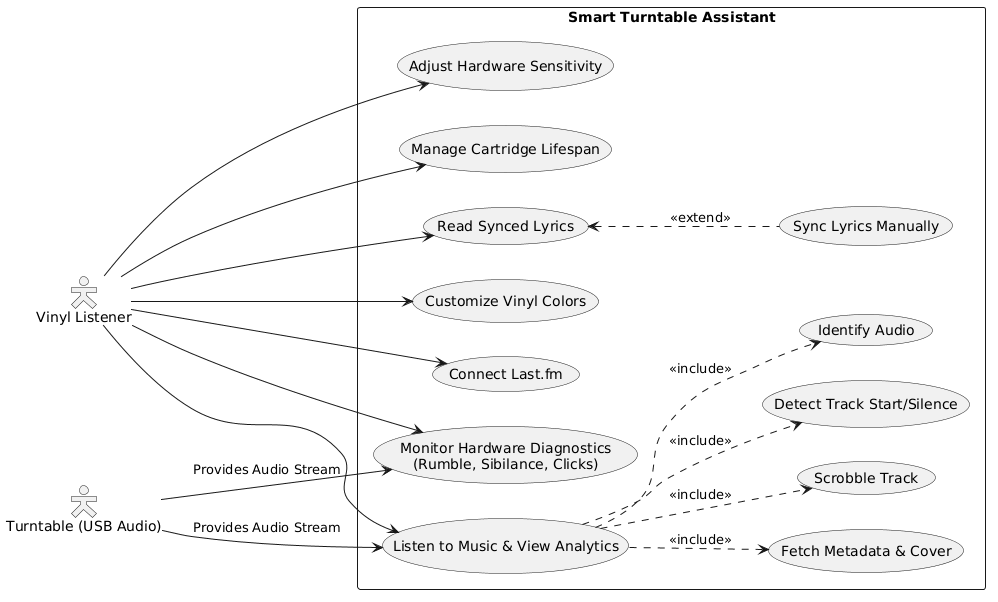
\includegraphics[width=0.8\textwidth]{Images/usecase.png}
    \caption{UML Use Case Diagram}
    \label{fig:usecase}
\end{figure}

\begin{figure}[htbp]
    \centering
    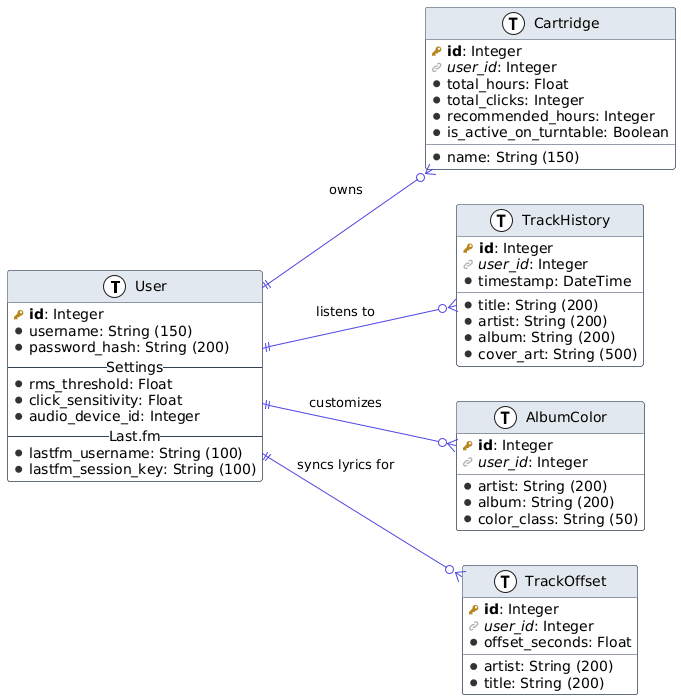
\includegraphics[width=0.85\textwidth]{Images/database.png}
    \caption{ER Diagram az adatbázis sémájáról}
    \label{fig:database}
\end{figure}

\begin{figure}[htbp]
    \centering
    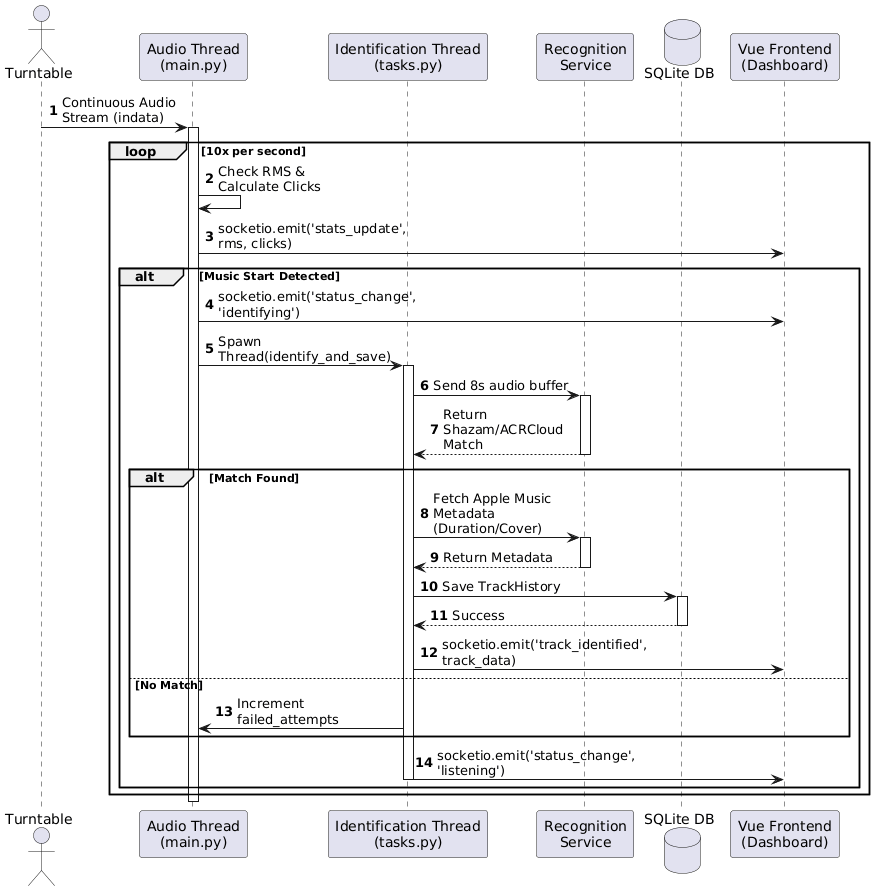
\includegraphics[width=1\textwidth]{Images/sequence.png}
    \caption{UML Sequence Diagram}
    \label{fig:sequence}
\end{figure}

\begin{figure}[htbp]
    \centering
    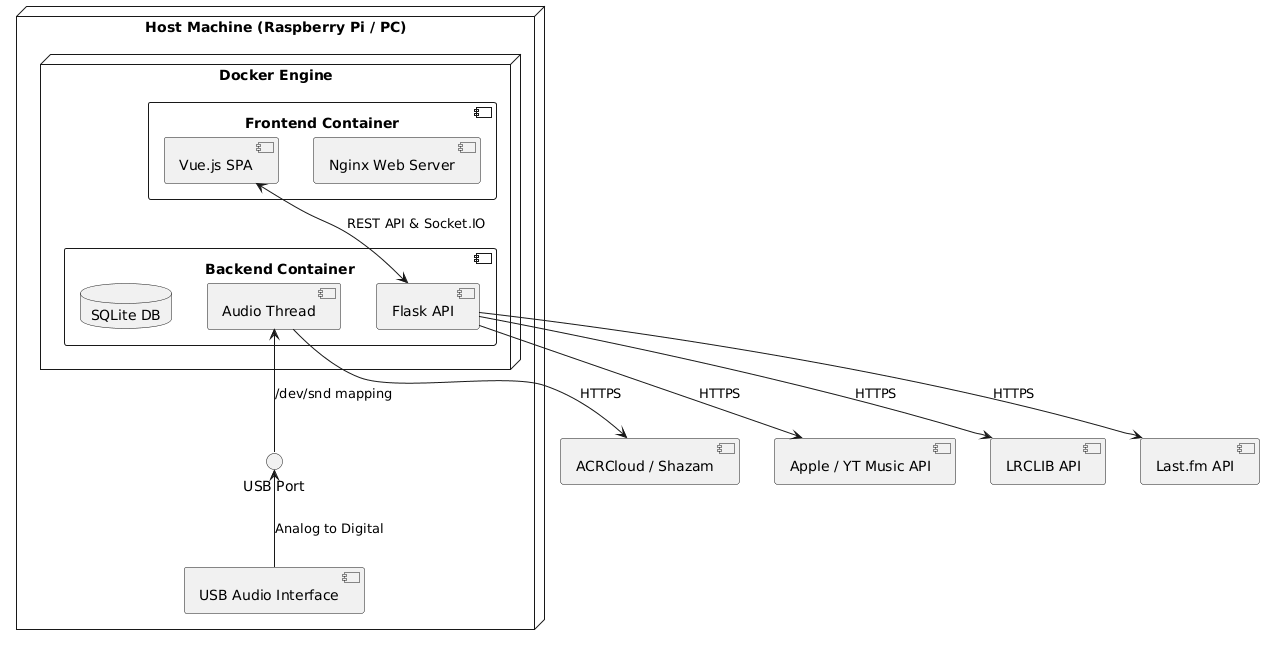
\includegraphics[width=1\textwidth]{Images/deployement.png}
    \caption{Deployment diagram amely a docker image felépítését mutatja be.}
    \label{fig:deployment}
\end{figure}

\end{document}